
\documentclass[10pt, a4paper]{article}
\usepackage{float} % display graphics at the demanded place
\usepackage{hyperref} % display table des matières
\usepackage{subcaption} % authorize subfigure
\usepackage{booktabs}
\usepackage[utf8]{inputenc}
\usepackage[T1]{fontenc}
%\usepackage[french]{babel} %casse tout chez moi
\usepackage{graphicx}

%élargi un peu pour que les diagrammes soient pas minuscules ou mal alignés
\evensidemargin=0in
\oddsidemargin=0in
\textwidth=6.5in

\graphicspath{{Diagrammes/}}


\title{INFO-F-109 : Projet d'informatique 2 \\
       \textbf{Software requirement document\\
	   Pawn Hub}}
\author{Huward Maxence, Boonen Jacques\\
		Pham Hong Phuc, Duc Nguyen, Caroline Forest\\
		Antunes Andre, Romain Mardulyn}
\date{}
\begin{document}
	\maketitle
	\tableofcontents %do a table of content automatically	
	\newpage
	\section{Introduction}
		\subsection{Description du projet}
			\paragraph{}L'objectif de ce projet est de recréer un grand classique des jeux de plateau: les échecs. Le but est d'implémenter une plateforme multijoueurs permettant de jouer en ligne le jeu classique ainsi que ses variantes.
Les joueurs auront des comptes utilisateurs et pourront intéragir entre eux sur la plateforme.
En plus du jeu usuel 8x8, nous allons aussi inclure les variantes de : AliceChess, DarkChess et HordeChess.

		\subsection{Historique des modifications}
		
		\begin{table}[h!]
			\centering
			\begin{tabular}{|c|c|c|p{50mm}|}
				\hline
				 \textbf{version} & \textbf{date} & \textbf{auteur}  & \textbf{description} \\ \hline
				 1 & 4/12 & Pham Hong Phuc & Création du SRD en LaTex\\ \hline
				 1.1 & 6/12 & Caroline Forest & Ajout de diagrammes UML\\ \hline

\end{tabular}
			\caption*{Historique des modifications}
			\end{table}
%fin du tableau

%BESOINS UTILISATEURS%

	\section{Besoins utilisateurs}
		\subsection{Fonctionnels}
		
\begin{figure}[h]
\centering
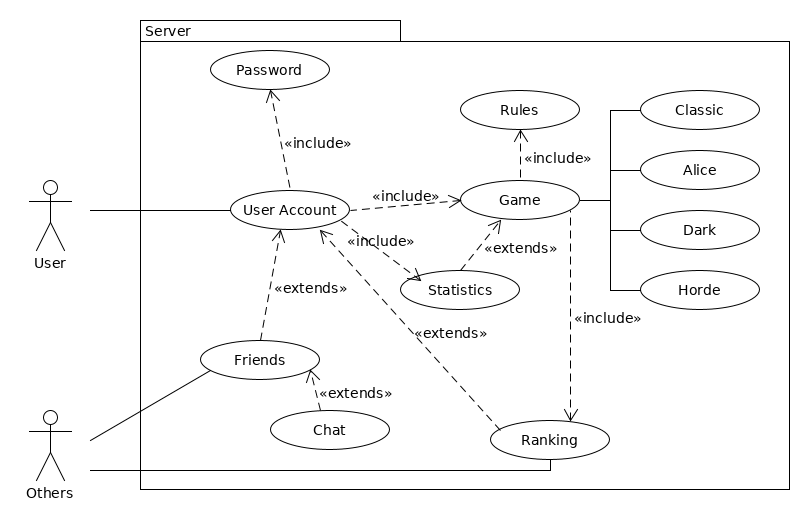
\includegraphics[scale=0.4]{Use_Case.png}
\caption{Diagramme de \textit{use case} des actions possibles d'un utilisateur}
\label{UC_act} %UseCase_actions
\end{figure}
		
		\subsection{Connexion}


		\subsection{Durant une partie}
		
		\subsection{Non-fonctionnels}
		
	\section{Besoins systèmes}
		\subsection{Fonctionnels}
		\subsubsection{Connexion au serveur}
		
		\subsubsection{Partie joueur vs. joueur}
		
		\subsection{Non-fonctionnel}
		
	\section{Design du système}
	
\begin{figure}[h]
\centering
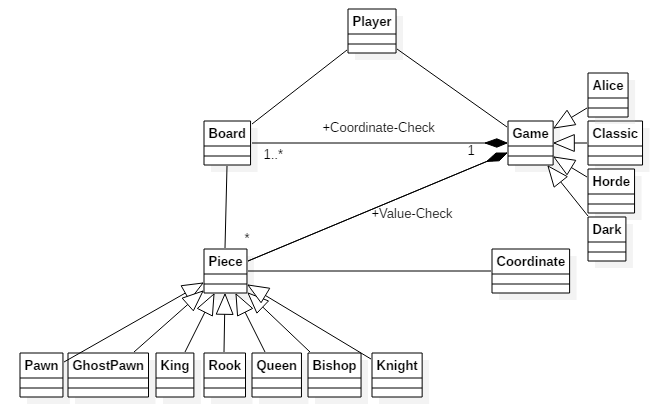
\includegraphics[scale=0.45]{ClassDiagram.png}
\caption{Diagramme de classes général}
\label{CD} %ClassDiagram
\end{figure}
		
		\subsection{Connexion du joueur}
		
		\subsection{Les actions du joueur}
		
		\subsection{Client-Serveur}
		\paragraph{}Le serveur aura une copie du board et se tâchera de devoir vérifier les différentes actions des joueurs. Il veillera également à  mettre à jour les board des joueurs.
		\subsection{Les modes de jeu}
		\paragraph{}Quatre modes sont proposés:
		
		\subsection{Menu}
		
	\section{Annexe}
	
	
		
		
		
		

\end{document}